\section{Introduction}

Drivers enter a parking lot without having any specific knowledge about the
lot's availability. It is not uncommon for any driver to spend an additional,
non-trivial amount of time looking for a parking spot. This searching time
directly translates into not only frustration but also wasted energy and carbon
dioxide harmful for the environment.

In order to assist drivers searching for a parking space, numerous smartphone
applications are available in the online application stores and many academic
systems have been proposed~\cite{4212497, Chen:2012:COS, Delot:2009:CRP,
5062057, Mathur:2010:PDS}. These applications and systems make a variety of
assumptions such as availability of additional infrastructure~\cite{5062057},
additional equipment deployed on vehicles monitored~\cite{Mathur:2010:PDS},
vehicular networks~\cite{Delot:2009:CRP, Mathur:2010:PDS, 4212497}, and manual
user reports~\cite{Chen:2012:COS}.

We present {\it PocketParker}, a system that predicts parking lot availability
using smartphones. Unlike previous approaches, our goal is to not require any
additional input or infrastructure other than the smartphones used by the users
of PocketParker. In order to accomplish this goal, we address two main
challenges. We accomplish this goal by combining an activity detector
deployed as a smartphone appplication that automatically extracts park and
depark events as well as a prediction model that estimates parking lot
availability based on observed events. Our activity detector addresses the
challenges of energy efficiency and accuracy of detection. Our prediction model
addresses the challenges of estimating the number of {\it hidden drivers} who do
not participate in PocketParker as well as arrival and departure rates of a
parking lot. Using this information, PocketParker probabilistically estimates
how many parking spots are available at any given time.

\begin{figure}
\centering
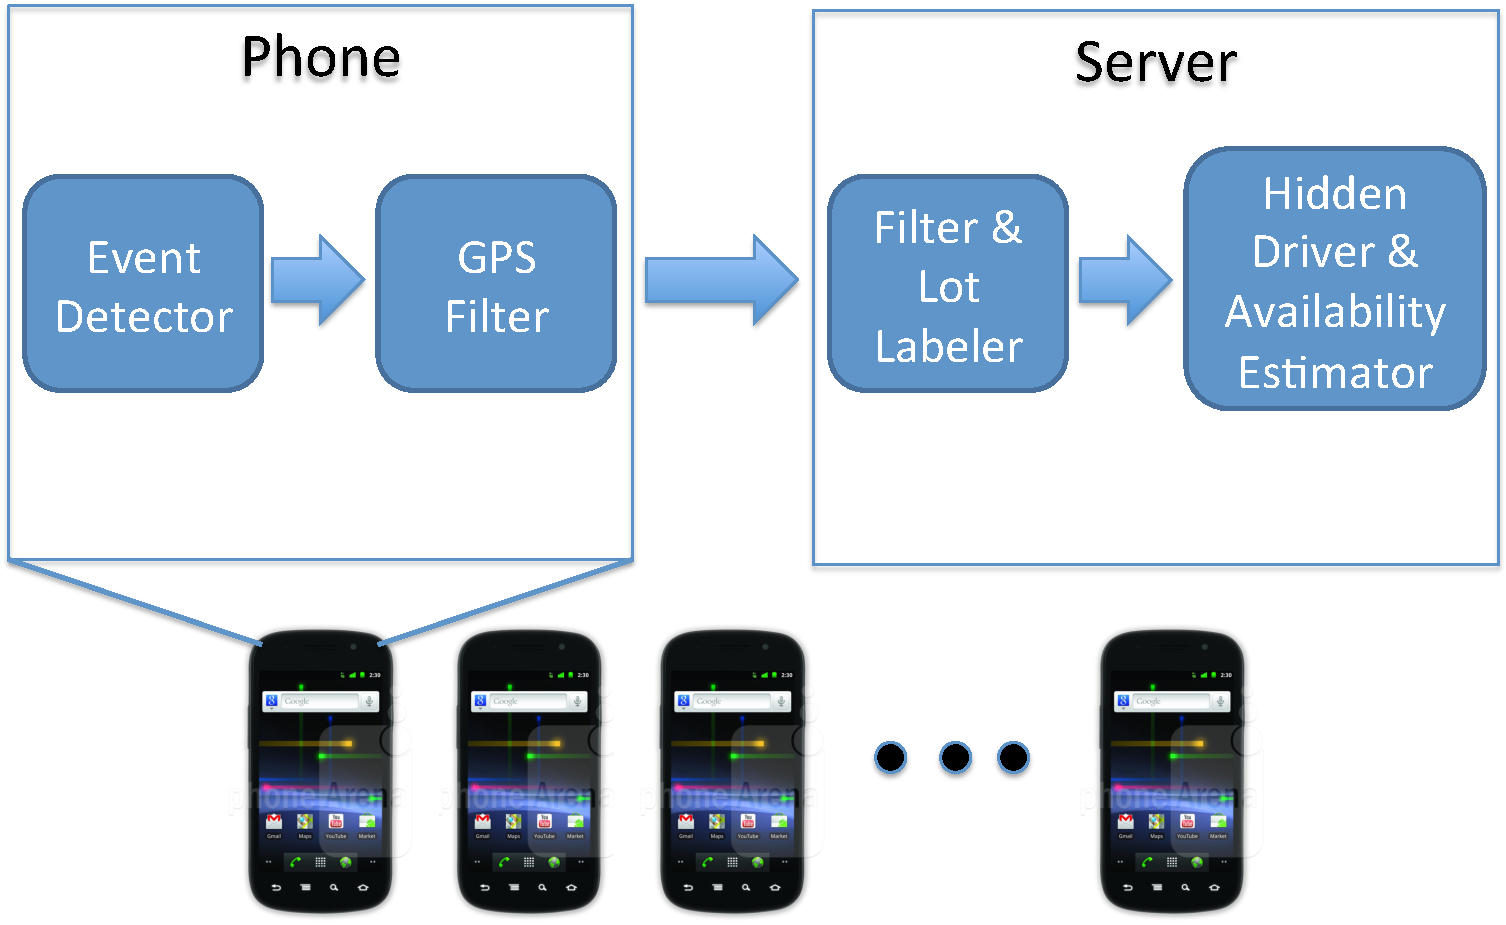
\includegraphics[width=\columnwidth]{./figures/blockdiagram.pdf}

\caption{\textbf{PocketParker architecture.}}

\label{fig-arch}
\end{figure}

\subsection{Usage Model}
